% vim: foldmethod=marker: 
\documentclass[11pt]{standalone}

\usepackage[utf8]{inputenc}
\usepackage[T1]{fontenc}    

\usepackage{amsmath}
\usepackage{amsfonts}
\usepackage{amssymb}
\usepackage{mathrsfs}

\usepackage{tikz}
\usetikzlibrary{snakes} %% produces curly arrows on tikz
\usetikzlibrary{matrix} %% for commutative diagrams
\usetikzlibrary{arrows}

\usetikzlibrary{shadings}
%\definecolor{azulClaro}{RGB}{65,105,225}
\definecolor{azulClaro}{RGB}{0, 102, 204}

\usetikzlibrary{fadings}

\tikzfading[name=fade out, inner color=transparent!0, outer color=transparent!100]

\begin{document}

    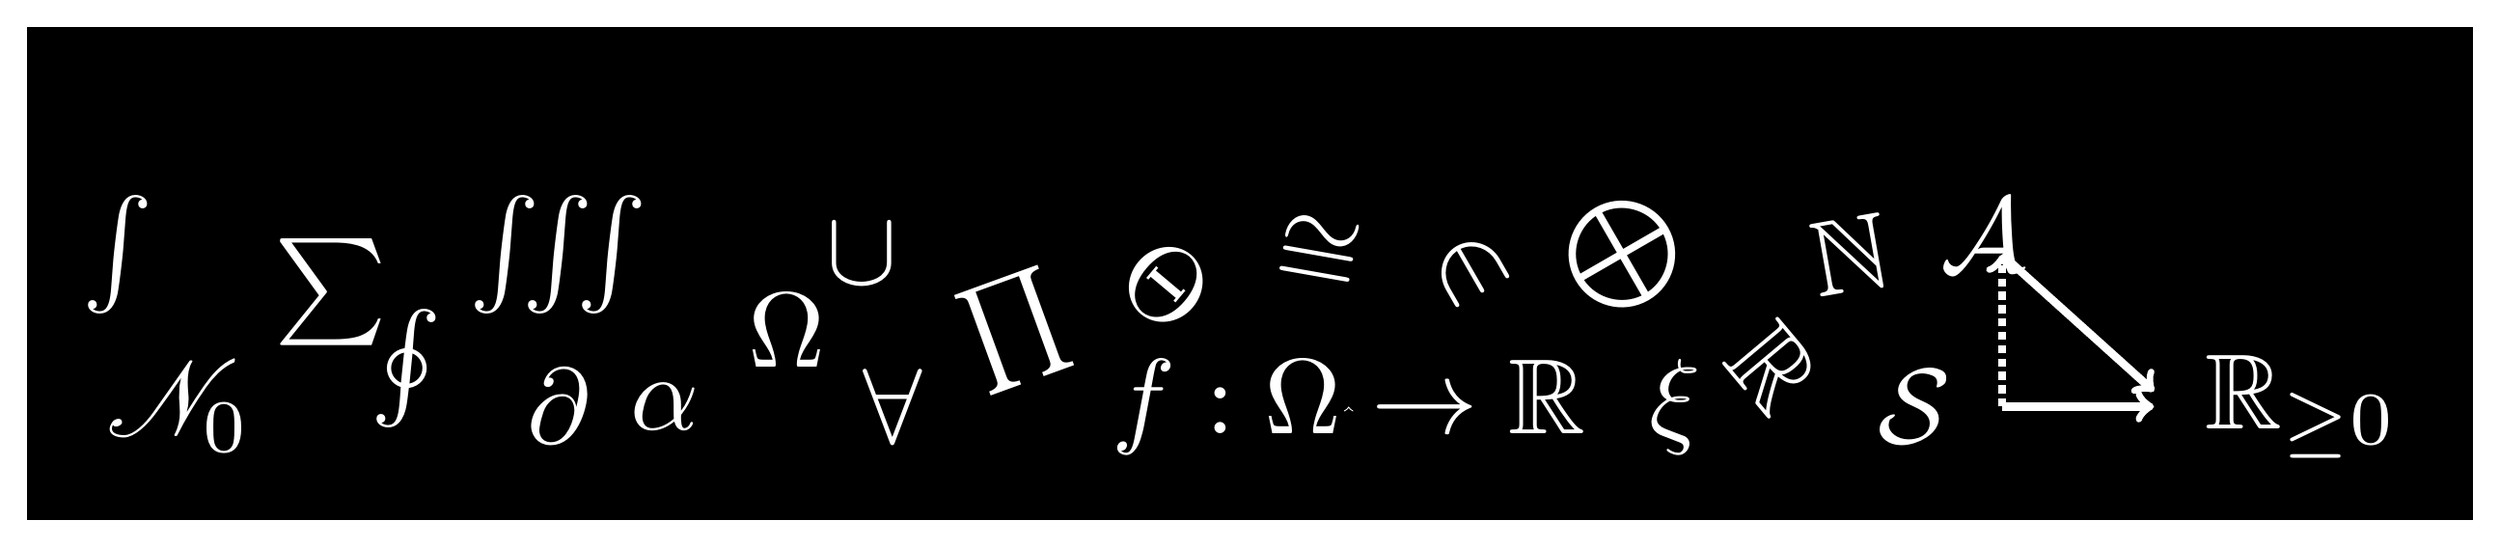
\begin{tikzpicture}

        \fill[black] (-22,-3.5) rectangle (10.2,3);

        \draw[white] (-20.8,0) node[scale=4] {$\int$};
        \draw[white] (-18,-0.5) node[scale=4] {$\sum$};
        \draw[white] (-15,0) node[scale=4,rotate=00] {$\iiint$};
        \draw[white] (-20,-2.0) node[scale=4] {$\mathscr{N}_0$};
        \draw[white] (-17,-1.5) node[scale=4] {$\oint$};
        \draw[white] (-15,-2) node[scale=4] {$\partial$};
        \draw[white] (-12,-1) node[scale=4] {$\Omega$};
        \draw[white] (-11,0) node[scale=4] {$\cup$};
        \draw[white] (-13.6,-2) node[scale=4,rotate=00] {$\alpha$};
        %\draw[white] (-9,-1) node[scale=4] {$\cap$};
        \draw[white] (-10.6,-2.0) node[scale=4,rotate=0] {$\forall$};
        \draw[white] (-9,-1) node[scale=4,rotate=20] {$\prod$};
        \draw[white] (-7.0,-0.4) node[scale=4,rotate=-40] {$\Theta$};
        \draw[white,->] (-4.6,-2.0) node[scale=4,rotate=0] {$f: \Omega \to \mathbb{R}$};
        \draw[white] (-5,0) node[scale=4,rotate=-10] {$\cong$};
        \draw[white] (-3,-0.2) node[scale=4,rotate=-60] {$\in$};
        \draw[white] (-1,0) node[scale=4,rotate=30] {$\bigoplus$};
        \draw[white] (-0.3,-2) node[scale=4,rotate=00] {$\xi$};
        \draw[white] (1,-1.5) node[scale=4,rotate=-50] {$\mathbb{R}$};
        \draw[white] (2,0) node[scale=4,rotate=10] {$\mathbb{N}$};
        %\draw[white] (3.5,0) node[scale=4,rotate=00] {$\mathbb{Z}$};
        %\draw[white] (5,0) node[scale=4,rotate=30] {$\mathbb{Q}$};
        %\draw[white] (3,-1.7) node[scale=4,rotate=30] {$\beta$};

        \draw[->,white, line width=3pt] (4,-2) node[scale=4,left] {$\mathcal{S}$} --
           (6,-2) node[scale=4, right] {$\mathbb{R}_{\geq 0}$};
        \draw[->,white, line width=3pt] (4,0) -- node[scale=4,above left] {$\mathcal{A}$}
            (6,-1.8);
        \draw[->,white, line width=3pt,  dotted] (4,-2) -- (4,0);



        



        

    \end{tikzpicture}

\end{document}


